\section{Experiments}
\label{sec:experiments}

We evaluate the algorithm of Section~\ref{sec:solution}, which we call \textsf{PrivExpl} here, on six datasets and $44$ query pairs covering query refinement, consistent query answering and contrasts; $27$ of the pairs come from earlier work.
The experiments answer three questions:
(1)~do the released explanations show an analyst something the two queries and the constraint do not (Section~\ref{sec:usecase-results});
(2)~how close do they come to the best non-private selection, and what limits them (Section~\ref{subsec:quality});
(3)~what does the algorithm cost in time (Section~\ref{subsec:scalability}).

% ---------------------------------------------------------------
\subsection{Setup}
\label{subsec:experimental-setup}

\begin{table}[t]
\centering
\small
\caption{Datasets and the source of their query pairs. On IPUMS-CPS $|\mathcal{P}|$ depends on the attribute each question removes.}
\label{tab:datasets}
\setlength{\tabcolsep}{3pt}
\resizebox{\columnwidth}{!}{\begin{tabular}{@{}lrrrlrl@{}}
\toprule
Dataset & $N$ & $|\Attrs|$ & $|\mathcal{P}|$ & Setting & Pairs & Pairs from \\
\midrule
Adult~\cite{adult-uci}            & 48{,}842    & 10 & 1{,}144 & refinement & 7  & ours \\
ACSIncome~\cite{DingHMS21}       & 1{,}664{,}500 & 10 & 1{,}084 & refinement & 10 & Erica~\cite{LMSJ23} \\
Tax~\cite{BohannonFGJK07}        & 200{,}000   & 9  & 2{,}106 & refinement & 4  & ours \\
Tax-dirty~\cite{MahdaviAFMOST19} & 200{,}000   & 9  & 2{,}300 & CQA        & 3  & ours, rules~\cite{NiMZWLY24} \\
Hospital~\cite{rekatsinas2017}   & 1{,}000     & 10 & 502     & CQA        & 3  & ours \\
IPUMS-CPS~\cite{TaoGMR22}        & 1{,}146{,}552 & 8 & 746--1{,}124 & contrast  & 17 & DPXPlain~\cite{TaoGMR22} \\
\bottomrule
\end{tabular}}
\end{table}

\paragraph{Datasets.}
Table~\ref{tab:datasets} summarises the six datasets, and Table~\ref{tab:attributes} (appendix) lists their attributes.
\begin{itemize}[leftmargin=*,itemsep=1pt,topsep=2pt]
  \item \textbf{Adult}~\cite{adult-uci} (real data): $48{,}842$ census records with $10$ explanation attributes. Seven refinement pairs of ours, including the running example A2.
  \item \textbf{ACSIncome}~\cite{DingHMS21} (real data): $1{,}664{,}500$ records of the American Community Survey, the dataset of Erica~\cite{LMSJ23,ERICA}. Ten refinement pairs from Erica.
  \item \textbf{Tax}~\cite{BohannonFGJK07} (synthetic data): the $200{,}000$-tuple clean file of Raha~\cite{MahdaviAFMOST19}. Four refinement pairs of ours.
  \item \textbf{Tax-dirty}~\cite{MahdaviAFMOST19} (synthetic data, injected errors): the dirty file of the same Tax data, with the Tax rules of Ni et~al.~\cite{NiMZWLY24}. Three CQA pairs of ours.
  \item \textbf{Hospital}~\cite{rekatsinas2017} (real data, injected errors): HoloClean's $1{,}000$-tuple dirty file with three functional dependencies (Table~\ref{tab:pairs}). Three CQA pairs of ours.
  \item \textbf{IPUMS-CPS}~\cite{TaoGMR22} (real data): DPXPlain's extract of the Current Population Survey, $1{,}146{,}552$ tuples. All $17$ contrast questions of DPXPlain.
\end{itemize}
Numeric attributes are bucketed into equal-width bins with rounded edges: ages and weekly hours by decade, a separate bin for $0$ where most values are $0$, and the education code of ACSIncome by level.
In the dirty files, missing and out-of-domain values go to \texttt{NA} and \texttt{Other} bins.
Views are conjunctions of at most two conditions.

\paragraph{Query pairs.}
Table~\ref{tab:pairs} lists the $44$ pairs, $27$ of them from earlier work.
\begin{itemize}[leftmargin=*,itemsep=1pt,topsep=2pt]
  \item \emph{Refinement}: $Q_2$ changes predicates of $Q_1$ so that its output meets a constraint on the representation of a group.
  \item \emph{CQA}: $Q_2=Q_\Sigma$ is the consistent answer of $Q_1$ under the integrity constraints of the dataset.
  \item \emph{Contrast}: $Q_1$ and $Q_2$ select two disjoint groups of the same table.
\end{itemize}
Section~\ref{sec:usecase-results} describes how the pairs of each setting were built.
The explanations depend only on the two selections, so Table~\ref{tab:pairs} omits the aggregates the analyst compares (e.g.\ \texttt{AVG(Rate)} in D1).

% generated by `python -m pqde.paper_tables` from configs/ and results/e1/summary.csv -- do not edit
\begin{table*}[t]
\centering
\scriptsize
\caption{The 46 query pairs of the experiments, by dataset; the 10 pairs of the Erica experiments (last three groups) serve for running time only. Bold: the case studies of Section~\ref{sec:usecase-results}. ACS codes are shown by name; \texttt{SCHL} 16 = high-school diploma, 19 = some college, 21 = bachelor's, 22 = master's, 23 = professional degree.}
\label{tab:pairs}
\setlength{\tabcolsep}{3pt}
\renewcommand{\arraystretch}{1.08}
\begin{tabularx}{\textwidth}{@{}l>{\raggedright\arraybackslash}X>{\raggedright\arraybackslash}X>{\raggedright\arraybackslash}p{4.4cm}@{}}
\toprule
ID & $Q_1$ & $Q_2$ & Constraint\\
\midrule
\multicolumn{4}{@{}p{\textwidth}@{}}{\emph{Adult~\cite{adult-uci}: refinements under representation constraints (ours); A2 is the running example of Section~\ref{sec:introduction}.}}\\[1pt]
A1 & \texttt{occupation = Craft-repair $\wedge$ hoursPerWeek$\,\ge\,$40} & \texttt{occupation IN (Adm-clerical, Craft-repair) $\wedge$ hoursPerWeek$\,\ge\,$40} & $\ge$25\% \texttt{gender = Female} \\
\textbf{A2} & \texttt{education IN (Bachelors, Masters) $\wedge$ hoursPerWeek$\,\ge\,$50} & \texttt{education = Masters $\wedge$ hoursPerWeek$\,\ge\,$30} & $\ge$25\% \texttt{gender = Female} \\
A3 & \texttt{maritalStatus = Married-civ-spouse $\wedge$ hoursPerWeek$\,\ge\,$45} & \texttt{maritalStatus IN (Divorced, Married-civ-spouse, Never-married) $\wedge$ hoursPerWeek$\,\ge\,$38} & $\ge$25\% \texttt{gender = Female} \\
A4 & \texttt{education IN (Masters, Doctorate, Prof-school) $\wedge$ hoursPerWeek$\,\ge\,$50} & \texttt{education IN (Doctorate, Masters, Prof-school, Some-college) $\wedge$ hoursPerWeek$\,\ge\,$35} & $\ge$30\% \texttt{gender = Female} \\
A5 & \texttt{occupation = Prof-specialty $\wedge$ maritalStatus = Married-civ-spouse} & \texttt{occupation IN (Other-service, Prof-specialty) $\wedge$ maritalStatus IN (Married-civ-spouse, Never-married)} & $\ge$15\% \texttt{race IN (Black, Asian-Pac-Islander, Amer-Indian-Eskimo, Other)} \\
A6 & \texttt{maritalStatus = Married-civ-spouse $\wedge$ age$\,\ge\,$40} & \texttt{maritalStatus IN (Divorced, Married-civ-spouse, Widowed) $\wedge$ age$\,\ge\,$61} & $\ge$30\% \texttt{gender = Female} \\
A7 & \texttt{occupation = Prof-specialty $\wedge$ hoursPerWeek$\,\ge\,$50} & \texttt{occupation IN (Other-service, Prof-specialty) $\wedge$ hoursPerWeek$\,\ge\,$30} & $\ge$25\% \texttt{age$\,<\,$30} \\
\midrule
\multicolumn{4}{@{}p{\textwidth}@{}}{\emph{ACSIncome~\cite{DingHMS21}: queries, constraints and refinements of Erica~\cite{LMSJ23}: the ten of its twelve query--constraint combinations whose refinement satisfies the constraints and, where Erica returns several refinements, the one that most changes the attributes the query and the constraints do not mention.}}\\[1pt]
\textbf{S1} & \texttt{WKHP$\,\ge\,$40 $\wedge$ SCHL$\,\ge\,$19 $\wedge$ COW IN (local-gov, state-gov, federal-gov)} & \texttt{WKHP$\,\ge\,$40 $\wedge$ SCHL$\,\ge\,$19 $\wedge$ COW IN (local-gov, state-gov, federal-gov, private)} & $\ge$48{,}884 \texttt{SEX = F $\wedge$ MAR = married}; $\ge$15{,}719 \texttt{RAC1P = Black} \\
S2 & \texttt{WKHP$\,\ge\,$40 $\wedge$ SCHL$\,\ge\,$19 $\wedge$ COW IN (local-gov, state-gov, federal-gov)} & \texttt{WKHP$\,\ge\,$41 $\wedge$ SCHL$\,\ge\,$19 $\wedge$ COW IN (local-gov, state-gov, federal-gov)} & $\le$15{,}249 \texttt{SEX = M $\wedge$ RELP = spouse}; $\le$11{,}498 \texttt{age\_bucket = 30-60 $\wedge$ MAR = divorced} \\
S3 & \texttt{WKHP$\,\le\,$40 $\wedge$ SCHL$\,\le\,$19 $\wedge$ PINCP\_bucket IN ($<$20K, 20K-40K)} & \texttt{WKHP$\,\le\,$40 $\wedge$ SCHL$\,\le\,$19 $\wedge$ PINCP\_bucket IN ($<$20K, 20K-40K, 40K-60K)} & $\ge$125{,}492 \texttt{SEX = F $\wedge$ MAR = married}; $\ge$69{,}207 \texttt{RAC1P = Black} \\
S4 & \texttt{WKHP$\,\le\,$40 $\wedge$ SCHL$\,\le\,$19 $\wedge$ PINCP\_bucket IN ($<$20K, 20K-40K)} & \texttt{WKHP$\,\le\,$39 $\wedge$ SCHL$\,\le\,$19 $\wedge$ PINCP\_bucket IN ($<$20K, 20K-40K)} & $\le$33{,}674 \texttt{SEX = M $\wedge$ RELP = spouse}; $\le$36{,}921 \texttt{age\_bucket = 30-60 $\wedge$ MAR = divorced} \\
S5 & \texttt{WKHP$\,\le\,$40 $\wedge$ SCHL$\,\le\,$19 $\wedge$ PINCP\_bucket IN ($<$20K, 20K-40K)} & \texttt{WKHP$\,\le\,$38 $\wedge$ SCHL$\,\le\,$22 $\wedge$ PINCP\_bucket IN ($<$20K, 20K-40K, $>$60K)} & $\ge$125{,}492 \texttt{SEX = F $\wedge$ MAR = married}; $\le$9{,}628 \texttt{SEX = M $\wedge$ RAC1P = Asian} \\
S6 & \texttt{WKHP$\,\ge\,$60 $\wedge$ SCHL$\,\le\,$16 $\wedge$ PINCP\_bucket = $<$20K} & \texttt{WKHP$\,\ge\,$60 $\wedge$ SCHL$\,\le\,$16 $\wedge$ PINCP\_bucket IN ($<$20K, $>$60K)} & $\ge$1{,}307 \texttt{SEX = F}; $\ge$521 \texttt{RAC1P = Black} \\
S7 & \texttt{WKHP$\,\ge\,$60 $\wedge$ SCHL$\,\le\,$16 $\wedge$ PINCP\_bucket = $<$20K} & \texttt{WKHP$\,\ge\,$60 $\wedge$ SCHL$\,\le\,$15 $\wedge$ PINCP\_bucket = $<$20K} & $\le$2{,}829 \texttt{RAC1P = White}; $\le$2{,}280 \texttt{age\_bucket = 30-60} \\
S8 & \texttt{WKHP$\,\ge\,$60 $\wedge$ SCHL$\,\le\,$16 $\wedge$ PINCP\_bucket = $<$20K} & \texttt{WKHP$\,\ge\,$66 $\wedge$ SCHL$\,\le\,$21 $\wedge$ PINCP\_bucket = $<$20K} & $\ge$521 \texttt{RAC1P = Black}; $\le$2{,}280 \texttt{age\_bucket = 30-60} \\
S9 & \texttt{WKHP$\,\ge\,$60 $\wedge$ SCHL$\,\ge\,$22 $\wedge$ PINCP\_bucket = $>$60K $\wedge$ COW IN (self-emp-not-inc, self-emp-inc)} & \texttt{WKHP$\,\ge\,$60 $\wedge$ SCHL$\,\ge\,$21 $\wedge$ PINCP\_bucket = $>$60K $\wedge$ COW IN (self-emp-not-inc, self-emp-inc)} & $\ge$552 \texttt{SEX = F}; $\ge$97 \texttt{RAC1P = Black}; $\ge$239 \texttt{MAR = divorced} \\
S10 & \texttt{WKHP$\,\ge\,$60 $\wedge$ SCHL$\,\ge\,$22 $\wedge$ PINCP\_bucket = $>$60K $\wedge$ COW IN (self-emp-not-inc, self-emp-inc)} & \texttt{WKHP$\,\ge\,$60 $\wedge$ SCHL$\,\ge\,$23 $\wedge$ PINCP\_bucket = $>$60K $\wedge$ COW IN (self-emp-not-inc, self-emp-inc)} & $\le$1{,}862 \texttt{RAC1P = White}; $\le$1{,}727 \texttt{SEX = M} \\
\midrule
\multicolumn{4}{@{}p{\textwidth}@{}}{\emph{Tax~\cite{BohannonFGJK07,MahdaviAFMOST19}: refinements under representation constraints (ours).}}\\[1pt]
T1 & \texttt{Rate$\,\ge\,$6 $\wedge$ HasChild = Y} & \texttt{Rate$\,\ge\,$5 $\wedge$ HasChild = Y} & $\ge$30\% \texttt{Salary$\,\le\,$40000} \\
T2 & \texttt{MaritalStatus = S $\wedge$ HasChild = N $\wedge$ Salary$\,\ge\,$50000} & \texttt{MaritalStatus = S $\wedge$ Salary$\,\ge\,$50000} & $\ge$30\% \texttt{HasChild = Y} \\
T3 & \texttt{Salary$\,\ge\,$60000 $\wedge$ Rate$\,\le\,$2} & \texttt{Salary$\,\ge\,$60000 $\wedge$ Rate$\,\le\,$3.9} & $\ge$40\% \texttt{Rate$\,>\,$0} \\
T4 & \texttt{Salary$\,\le\,$30000 $\wedge$ Rate$\,\le\,$2} & \texttt{Salary$\,\le\,$30000 $\wedge$ Rate$\,\le\,$3.1799998} & $\ge$50\% \texttt{Rate$\,>\,$0} \\
\midrule
\multicolumn{4}{@{}p{\textwidth}@{}}{\emph{COMPAS~\cite{compas-propublica}: refinements under representation constraints on the attributes and groups of the Erica experiments~\cite{ERICA} (ours).}}\\[1pt]
\textbf{C1} & \texttt{priors\_count$\,\ge\,$7} & \texttt{priors\_count$\,\ge\,$2} & $\ge$30\% \texttt{race = Caucasian} \\
C2 & \texttt{priors\_count$\,\ge\,$4 $\wedge$ c\_charge\_degree = felony} & \texttt{priors\_count$\,\ge\,$1 $\wedge$ c\_charge\_degree = felony} & $\ge$30\% \texttt{race = Caucasian} \\
C3 & \texttt{decile\_score$\,\ge\,$7 $\wedge$ c\_charge\_degree = felony} & \texttt{decile\_score$\,\ge\,$2 $\wedge$ c\_charge\_degree = felony} & $\ge$30\% \texttt{race = Caucasian} \\
C4 & \texttt{decile\_score$\,\ge\,$7 $\wedge$ is\_recid = yes} & \texttt{decile\_score$\,\ge\,$5} & $\ge$18\% \texttt{sex = Female} \\
C5 & \texttt{priors\_count$\,\ge\,$2 $\wedge$ is\_recid = yes} & \texttt{priors\_count$\,\ge\,$4 $\wedge$ is\_recid = yes} & $\ge$19\% \texttt{age\_cat = Greater than 45} \\
\midrule
\multicolumn{4}{@{}p{\textwidth}@{}}{\emph{Law Students~\cite{lsac-wightman98}: the dataset of~\cite{CSSM24}, refinements under representation constraints (ours).}}\\[1pt]
L1 & \texttt{LSAT$\,\ge\,$40 $\wedge$ region\_first IN (NE, GL)} & \texttt{LSAT$\,\ge\,$29 $\wedge$ region\_first IN (NE, GL)} & $\ge$6\% \texttt{race IN (Black, Hispanic, Mexican, Puertorican, Amerindian)} \\
L2 & \texttt{UGPA$\,\ge\,$3.5 $\wedge$ region\_first IN (NE, GL)} & \texttt{UGPA$\,\ge\,$2.9 $\wedge$ region\_first IN (NE, GL)} & $\ge$6\% \texttt{race IN (Black, Hispanic, Mexican, Puertorican, Amerindian)} \\
L3 & \texttt{sander\_index$\,\ge\,$0.8 $\wedge$ region\_first IN (NE, GL)} & \texttt{sander\_index$\,\ge\,$0.629761905 $\wedge$ region\_first IN (NE, GL)} & $\ge$6\% \texttt{race IN (Black, Hispanic, Mexican, Puertorican, Amerindian)} \\
L4 & \texttt{LSAT$\,\ge\,$40 $\wedge$ region\_first IN (FW, SE, SC)} & \texttt{LSAT$\,\ge\,$30 $\wedge$ region\_first IN (FW, SE, SC)} & $\ge$3\% \texttt{race = Black} \\
L5 & \texttt{sander\_index$\,\ge\,$0.8 $\wedge$ region\_first IN (FW, SE, SC)} & \texttt{sander\_index$\,\ge\,$0.651190476 $\wedge$ region\_first IN (FW, SE, SC)} & $\ge$3\% \texttt{race = Black} \\
\midrule
\multicolumn{4}{@{}p{\textwidth}@{}}{\emph{MEPS~\cite{meps-hc181}: refinements under representation constraints (ours).}}\\[1pt]
M1 & \texttt{UTILIZATION$\,\ge\,$20} & \texttt{UTILIZATION$\,\ge\,$8} & $\ge$35\% \texttt{AGE$\,<\,$45} \\
M2 & \texttt{TOTEXP$\,\ge\,$5000 $\wedge$ HIBPDX = yes} & \texttt{TOTEXP$\,\ge\,$523 $\wedge$ HIBPDX = yes} & $\ge$44\% \texttt{SEX = M} \\
M3 & \texttt{HIBPDX = yes $\wedge$ INSCOV = public only} & \texttt{HIBPDX = yes $\wedge$ INSCOV IN (private, public only)} & $\ge$44\% \texttt{SEX = M} \\
M4 & \texttt{UTILIZATION$\,\ge\,$10 $\wedge$ RTHLTH IN (fair, poor)} & \texttt{UTILIZATION$\,\ge\,$4 $\wedge$ RTHLTH IN (fair, poor)} & $\ge$50\% \texttt{RACE IN (Black, Hispanic)} \\
M5 & \texttt{TOTEXP$\,\ge\,$5000 $\wedge$ INSCOV = public only} & \texttt{TOTEXP$\,\ge\,$2019 $\wedge$ INSCOV = public only} & $\ge$35\% \texttt{AGE$\,<\,$45} \\
\midrule
\multicolumn{4}{@{}p{\textwidth}@{}}{\emph{Adult, the copy of the Erica experiments~\cite{ERICA} ($32{,}561$ tuples): their queries and constraints, and the stored refinement closest to $Q_1$; running time only.}}\\[1pt]
EA1 & \texttt{education\_num$\,\ge\,$12 $\wedge$ hours\_per\_week$\,\ge\,$21 $\wedge$ capital\_gain$\,\ge\,$5501} & \texttt{education\_num$\,\ge\,$12 $\wedge$ hours\_per\_week$\,\ge\,$21 $\wedge$ capital\_gain$\,\ge\,$2580} & $\ge$200 \texttt{sex = Female} \\
EA2 & \texttt{education\_num$\,\ge\,$14 $\wedge$ hours\_per\_week$\,\ge\,$21 $\wedge$ capital\_gain$\,\ge\,$5501} & \texttt{education\_num$\,\ge\,$14 $\wedge$ hours\_per\_week$\,\ge\,$21 $\wedge$ capital\_gain$\,\ge\,$0} & $\ge$200 \texttt{sex = Female} \\
EA3 & \texttt{education\_num$\,\ge\,$9 $\wedge$ hours\_per\_week$\,\ge\,$21 $\wedge$ capital\_gain$\,\ge\,$5501} & \texttt{education\_num$\,\ge\,$9 $\wedge$ hours\_per\_week$\,\ge\,$41 $\wedge$ capital\_gain$\,\ge\,$15025} & $\le$20 \texttt{sex = Female}; $\le$180 \texttt{sex = Male $\wedge$ race = White} \\
\midrule
\multicolumn{4}{@{}p{\textwidth}@{}}{\emph{COMPAS, the copy of the Erica experiments~\cite{ERICA} ($11{,}757$ tuples): their queries and constraints, and the stored refinement closest to $Q_1$; running time only.}}\\[1pt]
EC1 & \texttt{juv\_fel\_count$\,\ge\,$1 $\wedge$ decile\_score$\,\ge\,$1 $\wedge$ r\_charge\_degree = F} & \texttt{juv\_fel\_count$\,\ge\,$0 $\wedge$ decile\_score$\,\ge\,$1 $\wedge$ r\_charge\_degree = F} & $\ge$23 \texttt{race = Caucasian}; $\ge$15 \texttt{age\_cat = Greater than 45} \\
EC2 & \texttt{juv\_fel\_count$\,\ge\,$1 $\wedge$ decile\_score$\,\ge\,$5 $\wedge$ r\_charge\_degree = F} & \texttt{juv\_fel\_count$\,\ge\,$0 $\wedge$ decile\_score$\,\ge\,$5 $\wedge$ r\_charge\_degree = F} & $\ge$23 \texttt{race = Caucasian}; $\ge$15 \texttt{age\_cat = Greater than 45} \\
EC3 & \texttt{juv\_fel\_count$\,\le\,$4 $\wedge$ decile\_score$\,\ge\,$8 $\wedge$ c\_charge\_degree = O} & \texttt{juv\_fel\_count$\,\le\,$4 $\wedge$ decile\_score$\,\ge\,$7 $\wedge$ c\_charge\_degree = O} & $\ge$10 \texttt{race = Caucasian}; $\ge$15 \texttt{age\_cat = Greater than 45} \\
\midrule
\multicolumn{4}{@{}p{\textwidth}@{}}{\emph{Healthcare, the data of the Erica experiments~\cite{ERICA} ($887$ tuples): their queries and constraints, and the stored refinement closest to $Q_1$; running time only.}}\\[1pt]
EH1 & \texttt{income$\,\ge\,$200 $\wedge$ num\_children$\,\ge\,$3 $\wedge$ county IN (county2, county3)} & \texttt{income$\,\ge\,$182 $\wedge$ num\_children$\,\ge\,$3 $\wedge$ county IN (county2, county3)} & $\ge$10 \texttt{race = race3}; $\ge$3 \texttt{race = race1 $\wedge$ age\_group = group1} \\
EH2 & \texttt{income$\,\ge\,$150 $\wedge$ num\_children$\,\le\,$4 $\wedge$ complications$\,\le\,$8 $\wedge$ county IN (county2, county4)} & \texttt{income$\,\ge\,$135 $\wedge$ num\_children$\,\le\,$4 $\wedge$ complications$\,\le\,$8 $\wedge$ county IN (county2, county4)} & $\ge$37 \texttt{race = race2}; $\ge$14 \texttt{race = race1 $\wedge$ age\_group = group1} \\
EH3 & \texttt{income$\,\le\,$100 $\wedge$ complications$\,\ge\,$5 $\wedge$ num\_children$\,\ge\,$4} & \texttt{income$\,\le\,$134 $\wedge$ complications$\,\ge\,$5 $\wedge$ num\_children$\,\ge\,$4} & $\ge$8 \texttt{race = race2}; $\ge$13 \texttt{age\_group = group1} \\
EH4 & \texttt{income$\,\ge\,$200 $\wedge$ num\_children$\,\ge\,$3 $\wedge$ county IN (county2, county3)} & \texttt{income$\,\ge\,$318 $\wedge$ num\_children$\,\ge\,$3 $\wedge$ county IN (county2, county3)} & $\le$5 \texttt{race = race2}; $\le$283 \texttt{age\_group = group2} \\
\bottomrule
\end{tabularx}
\end{table*}

% CQA and contrast pairs, out of the experiments for now:
% \begin{table*}[t]
% \centering
% \scriptsize
% \ContinuedFloat
% \caption{The query pairs of the experiments (continued).}
% \setlength{\tabcolsep}{3pt}
% \renewcommand{\arraystretch}{1.08}
% \begin{tabularx}{\textwidth}{@{}l>{\raggedright\arraybackslash}X>{\raggedright\arraybackslash}X@{}}
% \toprule
% ID & $Q_1$ & $Q_2$\\
% \midrule
% \multicolumn{3}{@{}p{\textwidth}@{}}{\emph{Tax-dirty~\cite{MahdaviAFMOST19}: consistent answers under the Tax rules of~\cite{NiMZWLY24} (ours).}}\\[1pt]
% D1 & \texttt{State IN (AK, CA, HI, OR, WA)} & $Q_\Sigma$ \\
% D2 & \texttt{State IN (AL, KY, MS, TN) $\wedge$ HasChild = N} & $Q_\Sigma$ \\
% D3 & \texttt{State IN (AK, CA, HI, OR, WA) $\wedge$ Rate$\,\le\,$3} & $Q_\Sigma$ \\
% \midrule
% \multicolumn{3}{@{}p{\textwidth}@{}}{\emph{Hospital~\cite{rekatsinas2017}: consistent answers under $\texttt{HospitalName}\to\texttt{ZipCode}$, $\texttt{HospitalName}\to\texttt{PhoneNumber}$, $\texttt{ZipCode}\to\texttt{City}$ (ours).}}\\[1pt]
% H1 & \texttt{HospitalType = acute care hospitals} & $Q_\Sigma$ \\
% H2 & \texttt{{auto: EmergencyService}} & $Q_\Sigma$ \\
% H3 & \texttt{{auto: HospitalOwner}} & $Q_\Sigma$ \\
% \midrule
% \multicolumn{3}{@{}p{\textwidth}@{}}{\emph{IPUMS-CPS~\cite{TaoGMR22}: the questions of DPXPlain~\cite{TaoGMR22}; the attribute that defines the groups is excluded from views and explanation attributes.}}\\[1pt]
% I1 & \texttt{SEX = Male} & \texttt{SEX = Female} \\
% I2 & \texttt{RELATE = Spouse} & \texttt{RELATE = Head/householder} \\
% I3 & \texttt{RELATE = Spouse} & \texttt{RELATE = Unmarried partner} \\
% I4 & \texttt{RELATE = Head/householder} & \texttt{RELATE = Child} \\
% I5 & \texttt{RELATE = Head/householder} & \texttt{RELATE = Parent} \\
% I6 & \texttt{MARST = Married, spouse present} & \texttt{MARST = Never married/single} \\
% I7 & \texttt{MARST = Divorced} & \texttt{MARST = Never married/single} \\
% I8 & \texttt{RACE = White} & \texttt{RACE = Black} \\
% I9 & \texttt{RACE = Asian only} & \texttt{RACE = White} \\
% I10 & \texttt{CITIZEN = Born in U.S} & \texttt{CITIZEN = Not a citizen} \\
% I11 & \texttt{CITIZEN = Naturalized citizen} & \texttt{CITIZEN = Born in U.S} \\
% I12 & \texttt{CLASSWKR = Wage/salary, private} & \texttt{CLASSWKR = Self-employed, not incorporated} \\
% I13 & \texttt{CLASSWKR = Federal government employee} & \texttt{CLASSWKR = State government employee} \\
% I14 & \texttt{AGE = (40, 50]} & \texttt{AGE = (30, 40]} \\
% I15 & \texttt{AGE = (60, 70]} & \texttt{AGE = (20, 30]} \\
% I16 & \texttt{EDUC = Bachelor's degree} & \texttt{EDUC = High school diploma or equivalent} \\
% I17 & \texttt{EDUC = Master's degree} & \texttt{EDUC = Bachelor's degree} \\
% \bottomrule
% \end{tabularx}
% \end{table*}


\paragraph{Metrics.}
All measures use exact histograms, so the Laplace noise of the release (scale $2k/\epsilon_H$) does not enter them.
\begin{itemize}[leftmargin=*,itemsep=1pt,topsep=2pt]
  \item \emph{Score} $F^0_\lambda(E)$ of a set $E$ of $k$ candidates: the objective $F_w$ of Definition~\ref{def:setobj} with $w_j=\lambda^{j-1}$ and $\gamma=0$. It does not depend on a parameter of the mechanism but rewards changes in very small bins, so where it matters we also report the smoothed score $F^\gamma_\lambda$, with the pair's default $\gamma$.
  \item \emph{ApproxRatio} against a reference set $E_B$: $F^0_\lambda(E)/F^0_\lambda(E_B)$.
  \item \emph{Precision@k}: $|E\cap E_B|/k$.
  \item \emph{Attribute precision}: the overlap of the two multisets of explained attributes, divided by $k$. We read it against its chance level, for $k$ candidates drawn at random from the candidates of the exact top-$\tau$ views.
  \item \emph{Coverage}: the mean $\Cov$ (Eq.~\eqref{eq:coverage-proxy}) of the views of a set.
\end{itemize}

\paragraph{Baselines and competitors.}
No earlier system explains the difference between two query outputs with histograms under differential privacy.
The closest, DPXPlain~\cite{TaoGMR22}, explains the difference between two group aggregates with predicates, an output $F^0_\lambda$ cannot score.
We therefore compare \textsf{PrivExpl} with non-private references, each removing one more of its ingredients, and with two private competitors.
\begin{itemize}[leftmargin=*,itemsep=1pt,topsep=2pt]
  \item \Bone{} (no noise): the exact top-$\tau$ views by $\Use$, then $k$ greedy rounds by $\HD_\gamma\cdot\DivS$.
  \item \Bthree{} (no noise, no smoothing): greedy by $\HD$. By Proposition~\ref{prop:greedy-exact} it returns the maximum of $F^0_\lambda$ over the candidates of the exact top-$\tau$ views, which we call the \emph{filtered optimum}. It is not an upper bound on \textsf{PrivExpl}, whose noisy view stage can retain other views.
  \item \Btwo{} (exhaustive search over the same candidates): returned the same score as \Bthree{} on every pair and setting, as the proposition guarantees; we use it only for running time.
  \item \textsf{SingleStage} (private): Algorithm~\ref{alg:topk} on the candidates of all views, without a view stage. It selects by $\HD_\gamma\cdot\DivS$ alone, ignoring representativeness and coverage, and spends $\epsilon_P+\epsilon_S$ on the selection and $\epsilon_H$ on the release, with $\gamma$ from Eq.~\eqref{eq:gamma-rule} for $|\mathcal{P}||\Attrs|$ candidates.
  \item \textsf{Random} (private): $k$ candidates drawn uniformly, with no budget spent on the selection.
\end{itemize}
Since \Bone{} and \Bthree{} differ only in $\gamma$, $F^0_\lambda(\Bone)/F^0_\lambda(\Bthree)$ is the cost of smoothing; the ratio to \Bone{} is the effect of noise at fixed smoothing, and can exceed $1$ because \Bone{} does not maximise the unsmoothed score.

\paragraph{Default setting and runs.}
Unless stated otherwise: the whole dataset, every view, $k=5$, $\lambda=0.5$, $\epsilon=1$ split equally ($\epsilon_P=\epsilon_S=\epsilon_H=1/3$), $\gamma_R=N/100$, $\tau=15$ and $\gamma\approx150$ from Eqs.~\eqref{eq:tau-rule} and~\eqref{eq:gamma-rule}, and $\bar N=|D|$; derived constants follow their rules when $k$, $\epsilon$ or $\tau$ vary.
\begin{itemize}[leftmargin=*,itemsep=1pt,topsep=2pt]
  \item \emph{Accuracy}: a point of a pair averages $40$ private runs, and a point of a dataset averages its pairs; a mean over all $44$ pairs weights each dataset by its number of pairs ($17$ on IPUMS-CPS). Each experiment draws its own runs, so the default point can differ between experiments in the second decimal.
  \item \emph{Running time}: measured end to end, ten times per point, on $22$ pairs (A1, A2, A4, A6, S1, S4, S6, S9, T1--T4, D1--D3, H1--H3, I1, I6, I8, I12). A run is stopped at $30$ minutes, and a point that reaches the limit is run three times.
\end{itemize}
\alon{Running-time experiments with the new bins are running; replace Figures~\ref{fig:scalability} and~\ref{fig:attrs} (top row) and the numbers of Section~\ref{subsec:scalability} when they finish.}

% ---------------------------------------------------------------
\subsection{Case Studies}
\label{sec:usecase-results}

We take one pair per setting: the running example (A2), the first query--constraint combination of Erica (S1), the first Tax-dirty pair (D1) and DPXPlain's default question (I1).
For each we made ten releases at the defaults.
Each figure shows the five explanations of the first release.
Bars are released values and black ticks exact counts, which are not released; each panel shows at most the six bins with the largest exact difference, and its title gives how many of the ten releases contain the same explanation.
The percentages below are computed from exact counts.
The released values carry noise with a standard deviation of about $42$ per bar, small against most bars of S1, D1 and I1 but not against the smaller bars of A2.

\begin{figure*}[t]
\centering
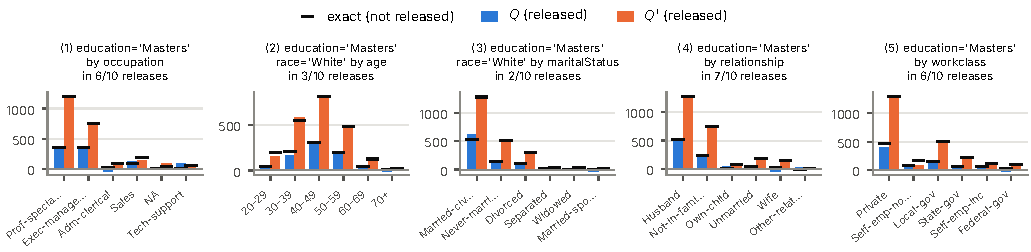
\includegraphics[width=\linewidth]{figures/exp/case_a2.pdf}
\caption{A2 (Adult, the running example): the five explanations of the first release.}
\label{fig:case-a2}
\end{figure*}

\paragraph{Refinement (A2): the Master's holders of the refined output differ in occupation, sector and marital status.}
Our refinement pairs on Adult and Tax come from a search for changes of one or two predicates of a query that meet a representation constraint (Table~\ref{tab:pairs}).
A2, the running example of Section~\ref{sec:introduction}, keeps only Master's degrees and lowers the hours threshold from $50$ to $30$, which raises the female share from $19.5\%$ to $30.6\%$.
The output shrinks from $3{,}055$ to $2{,}453$ tuples, and its Master's part grows from $874$ to all $2{,}453$.
Every release explains the Master's holders by occupation, relationship and workclass; the explanations of Figure~\ref{fig:case-a2} recur in two to seven of the ten releases.
Among them, the refined output has more professional-specialty workers ($41\%\rightarrow49\%$) and fewer executives ($41\%\rightarrow31\%$), more local and state government employees ($25\%\rightarrow30\%$), and fewer married members ($66\%\rightarrow59\%$ among white Master's holders).
The largest change, the $2{,}181$ Bachelor's holders that $Q_2$ drops ($71\%$ of $Q_1$), appears in only three releases, by hours worked.
$\HD_\gamma$ measures the change in each bin relative to the bin's support in the view, and $Q_1$ held only $27\%$ of the Bachelor's holders, while $Q_2$ adds $59\%$ of the Master's holders.

\begin{figure*}[t]
\centering
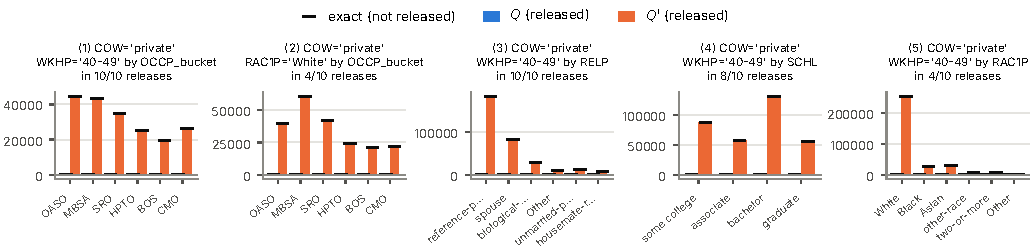
\includegraphics[width=\linewidth]{figures/exp/case_acs.pdf}
\caption{S1 (ACSIncome, from Erica): the five explanations of the first release. Occupation groups: OASO office and administrative support, MBSA management, SRO sales, HPTO healthcare practitioners, BOS business operations, CMO computer and mathematical.}
\label{fig:case-acs}
\end{figure*}

\paragraph{Refinement from Erica (S1): the release describes the workers the refinement adds.}
Erica~\cite{LMSJ23} computes minimal refinements of a query that meet cardinality constraints on groups.
On ACSIncome we use its queries and constraint sets with the refinements it returns, keeping the ten of its twelve query--constraint combinations whose refinement satisfies the constraints.
Where Erica returns several minimal refinements, we keep the one that most changes the attributes neither the query nor the constraints mention, which favours pairs with something to explain.
In S1, Erica meets the constraints on married women and Black workers by adding private-sector employees to a query over government employees; the output grows from $141{,}100$ to $587{,}712$.
In every release all five explanations are on private-sector views, which $Q_1$ does not meet (Figure~\ref{fig:case-acs}).
Among the added workers who work $40$--$49$ hours, $13\%$ are in office support, $13\%$ in management and $10\%$ in sales, $39\%$ hold a bachelor's degree, and $55\%$ are reference persons of their household.
An analyst comparing the incomes of the two outputs learns who was added, which the query, a change of one predicate, does not say.

\begin{figure*}[t]
\centering
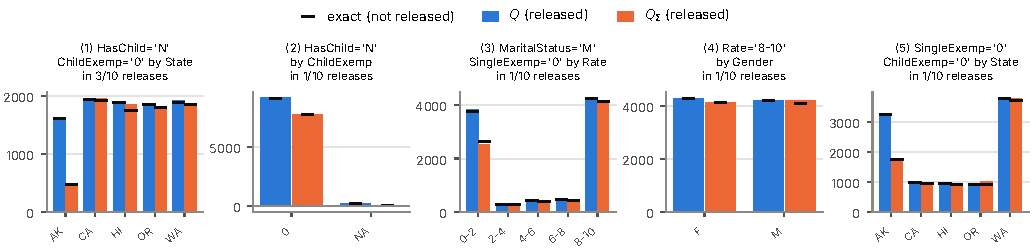
\includegraphics[width=\linewidth]{figures/exp/case_c1.pdf}
\caption{D1 (Tax-dirty, Pacific division, $Q_1$ against its consistent answer $Q_2=Q_\Sigma$): the five explanations of the first release.}
\label{fig:case-c1}
\end{figure*}

\paragraph{CQA (D1): the consistent answer loses half of Alaska, which raises the average rate.}
The consistent answer of a query under integrity constraints keeps the answers that hold in every repair~\cite{chomicki2004}; for a selection under subset repair (Definition~\ref{def:consistent-answer}), $Q_\Sigma(D)$ is $Q_1(D)$ minus the tuples in a conflict.
On Tax-dirty we use the Tax rules of Ni et~al.~\cite{NiMZWLY24} except $\texttt{AreaCode}\to\texttt{State}$, a rule written for cell repair that under subset repair puts $82\%$ of the tuples in conflict; with the other seven rules $3.9\%$ of the tuples are in conflict, unevenly across states.
Each of our CQA queries, on Tax-dirty and Hospital, is a selection whose consistent answer drops $10$--$90\%$ of its output, far more for some values than for others.
D1 selects the five Pacific states: $\texttt{AVG(Rate)}$ is $4.74$ on $Q_1(D)$ and $5.23$ on $Q_\Sigma(D)$, although $Q_\Sigma$ drops only $12\%$ of the tuples.
All ten releases explain the state, through one of three views (\texttt{HasChild}=\texttt{N} in six): Alaska loses half of its tuples, and $71\%$ of those with $\texttt{HasChild}=\texttt{N}$ and $\texttt{ChildExemp}=0$, while the other states lose at most $7\%$ (Figure~\ref{fig:case-c1}).
Every Alaska tuple has rate $0$, so dropping half of them raises the average.
Four releases also explain the rate: the lowest bin shrinks by $16$--$34\%$, the highest by at most $4\%$.

\begin{figure*}[t]
\centering
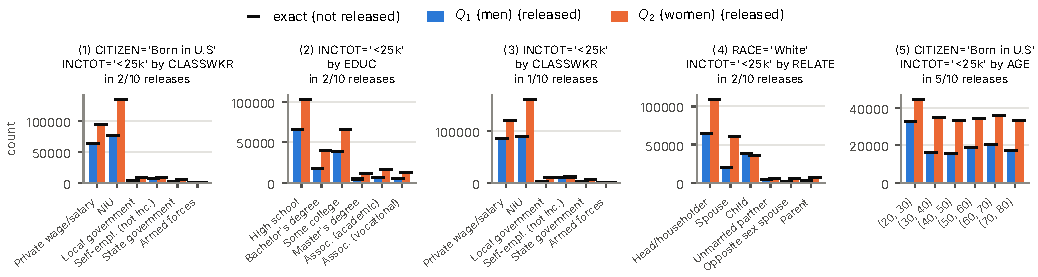
\includegraphics[width=\linewidth]{figures/exp/case_i1.pdf}
\caption{I1 (IPUMS-CPS, men against women): the five explanations of the first release. \texttt{NIU}: not in universe (not in the labour force).}
\label{fig:case-i1}
\end{figure*}

\paragraph{Contrast (I1): low-income women are more often spouses and outside the labour force than low-income men.}
In a contrast, $Q_1$ and $Q_2$ select two disjoint groups of the same table, the classical setting of contrast-set mining~\cite{BayPazzani01,DongLi99}, and the framework applies unchanged.
We use all $17$ questions of DPXPlain~\cite{TaoGMR22} on its IPUMS-CPS extract and remove the attribute that defines the two groups from the views and the explanation attributes, since it separates the groups by definition.
For DPXPlain's default question, I1, every release includes views on incomes under $25{,}000$, where women outnumber men $1.6$ to $1$ (Figure~\ref{fig:case-i1}).
Among them, women are more often outside the labour force ($52\%$ against $46\%$) and, among white respondents, the householder's spouse ($25\%$ against $14\%$); slightly more of them hold a bachelor's degree ($13\%$ against $9\%$).

% ---------------------------------------------------------------
\subsection{Explanation Quality}
\label{subsec:quality}

\begin{figure*}[t]
\centering
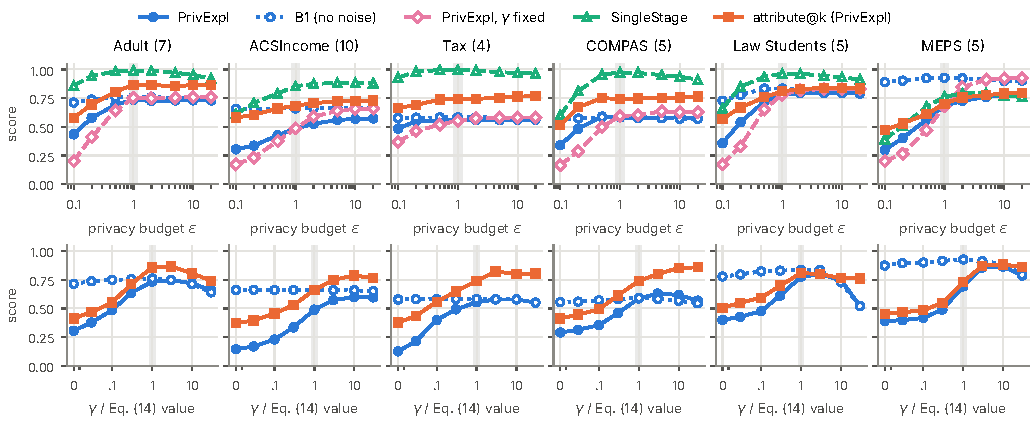
\includegraphics[width=\linewidth]{figures/exp/quality.pdf}
\caption{Quality against the privacy budget (top) and against $\gamma$ as a multiple of Eq.~\eqref{eq:gamma-rule} (bottom): ApproxRatio against the filtered optimum (solid) and against \Bone{} (dotted), attribute precision and precision@$k$; mean over the pairs of each dataset (number in parentheses), $40$ runs per pair and point. Shaded: defaults; the leftmost point of the bottom row is $\gamma=0$.}
\label{fig:quality}
\end{figure*}

\begin{figure*}[t]
\centering
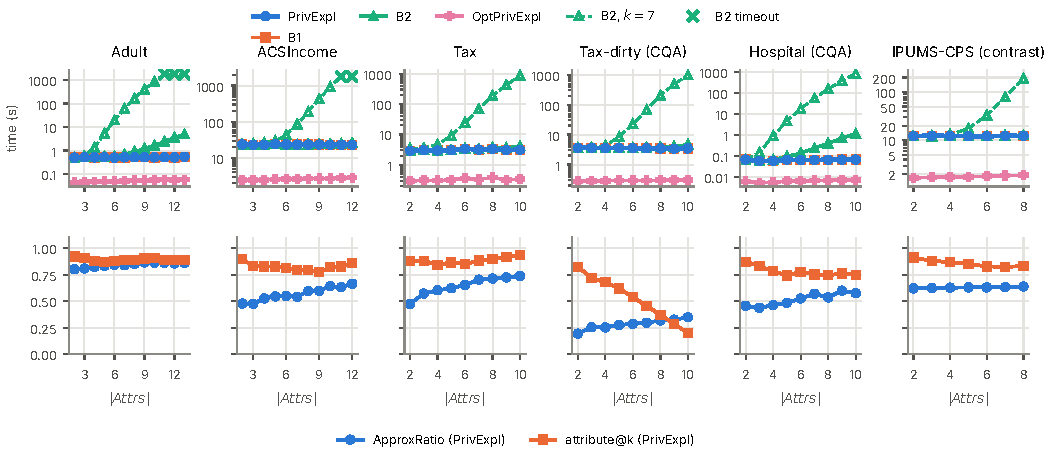
\includegraphics[width=\linewidth]{figures/exp/attrs.pdf}
\caption{The number of explanation attributes, from $2$ to every attribute of Table~\ref{tab:attributes}; views and reference attributes fixed. Each run draws its own random order of the attributes and keeps a prefix, so a point averages over random attribute sets of that size, not the default set. Top: running time (median of ten runs). Bottom: quality as in Figure~\ref{fig:quality} ($40$ runs per pair and point).}
\label{fig:attrs}
\end{figure*}

\begin{figure*}[t]
\centering
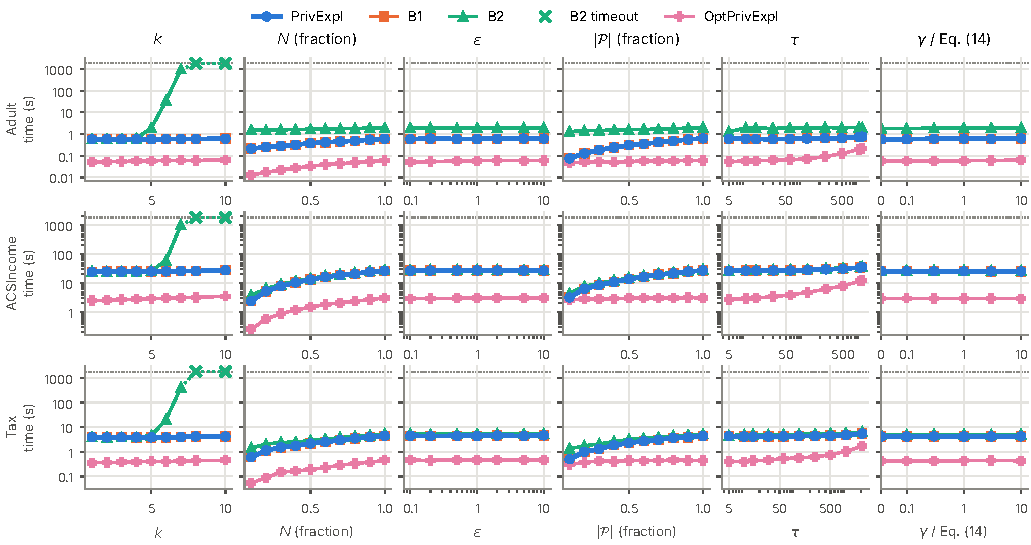
\includegraphics[width=\linewidth]{figures/exp/runtime_grid.pdf}
\caption{End-to-end running time (median of ten runs, mean over the dataset's runtime pairs), one parameter varied at a time. A cross marks a point stopped at the $30$-minute limit (three runs). Each row ran on its own machine.}
\label{fig:scalability}
\end{figure*}

\begin{table}[t]
\centering
\small
\caption{Quality of \textsf{PrivExpl} at the defaults ($\epsilon=1$), mean over the pairs of each dataset of the per-pair mean over $40$ runs. $F(\Bone)/F(\Bthree)$: cost of smoothing. Overlap measures against the filtered optimum; chance level of attribute precision in parentheses.}
\label{tab:quality}
\setlength{\tabcolsep}{3.5pt}
\begin{tabular}{@{}lccccc@{}}
\toprule
 & \multicolumn{2}{c}{ApproxRatio vs} & & & \\
\cmidrule(lr){2-3}
Dataset & \Bone{} & filt.\ opt. & $\frac{F(\Bone)}{F(\Bthree)}$ & Attr.\ prec. & Prec.@$k$\\
\midrule
Adult      & 1.00 & 0.96 & 0.95 & 0.79 (0.34) & 0.39\\
ACSIncome  & 0.80 & 0.80 & 1.00 & 0.72 (0.39) & 0.50\\
Tax        & 0.96 & 0.96 & 1.00 & 0.84 (0.32) & 0.52\\
Tax-dirty  & 0.66 & 0.64 & 0.98 & 0.56 (0.28) & 0.14\\
Hospital   & 0.67 & 0.55 & 0.80 & 0.52 (0.34) & 0.05\\
IPUMS-CPS  & 0.91 & 0.91 & 1.00 & 0.87 (0.46) & 0.35\\
\bottomrule
\end{tabular}
\end{table}

\paragraph{Three of the six datasets reach $0.91$--$0.96$ of the filtered optimum, with different explanations.}
\yuval{Start the section by describing the experiment: what did you run, and what question does it answer? The paragraph currently opens with numbers ("0.96 of the filtered optimum") before the reader knows the setting. Also consider a paragraph title that names the experiment (e.g., "Comparison with the non-private variants."). The current title is a long result claim that the reader can't yet interpret.}
At the defaults \textsf{PrivExpl} reaches $0.96$ of the filtered optimum on Adult and Tax and $0.91$ on IPUMS-CPS (Table~\ref{tab:quality})\yuval{When discussing a figure/table, open with "The results are shown in Table X / Figure Y" (and what is measured) before the numbers, rather than citing it in parentheses afterward.}, the datasets of $28$ of the $44$ pairs.
On IPUMS-CPS many candidates score alike, and even \textsf{Random} reaches $0.68$ (Table~\ref{tab:competitors}).
The scores hide that the explanations differ from the optimal ones\yuval{"Hide" sounds negative, as if the scores were misleading. Suggest: "A high score ratio does not mean the same explanations: …"}: on Adult \textsf{PrivExpl} holds $39\%$ of the optimal (view, attribute) pairs, on IPUMS-CPS $35\%$.
The leading candidates are near-ties (on Adult the best two differ by about $2\%$), typically a view and its refinement by one more condition explaining the same attribute\yuval{"Refinement" is overloaded. Use a different word, e.g., "a view and its specialization by one more condition" or "a view and a sub-view of it".}.
The attributes are mostly right: outside CQA, attribute precision is $0.72$--$0.87$, against a chance level of $0.32$--$0.46$\yuval{"Right" implies a ground truth. Here it means agreement with the filtered optimum. Say so directly, e.g., "The explained attributes mostly agree with the filtered optimum."}.
Two runs on the same pair thus return different sets of nearly equal scores.

\begin{figure}[t]
\centering
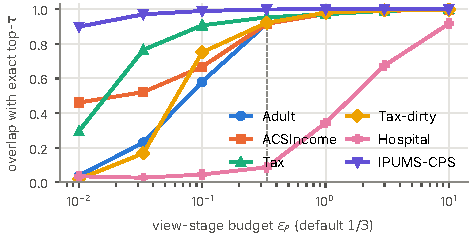
\includegraphics[width=\linewidth]{figures/exp/view_stage.pdf}
\caption{The view stage alone: overlap of the $\tau$ retained views with the exact top-$\tau$ by $\Use$ ($40$ runs per point).\yuval{Figure 11 is referenced only once (Tax-dirty, 5.3), and its content is never discussed. Either add a few sentences describing it, or drop the figure and keep the numbers you need in the text. If you keep it, place it after Figures 9 and 10 or renumber.}}
\label{fig:view-stage}
\end{figure}

\paragraph{Small differences and small data limit the explanation stage.}\yuval{Same here, start with the setting}
ACSIncome averages $0.80$ \yuval{Average of what? The same applies to "reaches 0.55" and "reaches 0.64" in this paragraph. Name the measure once per paragraph, at least.} because of three pairs at $0.33$--$0.45$ (S7, S8 and S10, all with outputs under $4{,}400$ tuples); the other seven reach $0.85$ or more.
Tax-dirty reaches $0.64$ although its view stage is accurate: $0.92$ of the retained views belong to the exact top-$\tau$ (Figure~\ref{fig:view-stage})\yuval{See my comment on the figure}.
Its best candidate scores $\HD_\gamma=0.62$ (median over runs), below the separation $2\ln|C_i|/((1+\gamma)\epsilon_i)\approx0.96$ that the mechanism resolves at the defaults; on the other datasets the best candidate scores $3.7$--$11$.
The draw is therefore spread over many candidates (precision@$k$ $0.14$), even though the relative gap between the two best candidates ($2.5\%$) is no smaller than on Adult.
Tax, on the same schema, reaches $0.96$; its pairs differ in $8.8$k--$58$k tuples, against $0.9$k--$2.3$k on Tax-dirty, which suggests that the size of the difference, more than the CQA setting, limits Tax-dirty.
Hospital ($N=1{,}000$) reaches $0.55$.
Its view stage retains $0.09$ of the exact top-$\tau$ on average and at most four of the fifteen in any release, against $0.91$ or more on the other datasets, as expected from a sensitivity of $4/\bar N$.
Its released histograms are of little use either: noise of scale $30$ exceeds most of its bins, and some released counts are negative.

\paragraph{Smoothing costs score only where bins are small, and data with large bins need more of it.}
Call the support $n_v$ of a candidate of a retained view in bin $v$ its bin size (Remark~\ref{rem:gamma-window}).
Smoothing alone costs \Bone{} $5\%$ on Adult, where $\gamma\approx150$ exceeds $82\%$ of the non-empty bins, and $20\%$ on Hospital ($99\%$); elsewhere at most $2\%$ (Table~\ref{tab:quality}).
On Adult \textsf{PrivExpl} scores as well as \Bone{} on average ($1.00$), so its gap to the filtered optimum comes from the smoothing rather than the noise.
Without smoothing the ApproxRatio drops from $0.85$ to $0.39$, and three or ten times the default raises it to $0.90$--$0.91$ (means over all $44$ pairs; bottom row of Figure~\ref{fig:quality}) \yuval{make it top row?}.
The default is the best multiple tried on Adult ($0.95$), but three times the default is best on Tax and Tax-dirty and ten times on ACSIncome and IPUMS-CPS.
There the median bin holds $680$--$940$ tuples, against $17$ on Adult, and the default $\gamma$ exceeds only $27\%$ (ACSIncome) and $4\%$ (Tax) of the bins.
A rule that adapts $\gamma$ to the bin sizes would need a private estimate of them; we leave it to future work.

\paragraph{With Eq.~\eqref{eq:gamma-rule}, more budget helps little on data with large bins.}\yuval{With Eq. (14)" is hard to parse as an opening: the reader has to remember what Eq. (14) does.}
Raising $\epsilon$ from $1$ to $20$ moves IPUMS-CPS only from $0.91$ to $0.92$ and ACSIncome from $0.80$ to $0.87$ (top row of Figure~\ref{fig:quality}), because the rule also lowers $\gamma$ ($150$, $30$ and $7.5$ at $\epsilon=1,5,20$).
With $\gamma$ fixed at its default value, both reach $0.97$--$1.00$ from $\epsilon=5$, and Tax-dirty $0.94$--$0.98$\yuval{Where are these shown? Cite the figure/table.}.
On Hospital, with its small bins, the rule does better ($0.94$ at $\epsilon=20$ against $0.81$), and below $\epsilon=1$ the fixed value is too small for the noise everywhere ($0.49$ against $0.66$ at $\epsilon=0.1$, mean over all $44$ pairs).\yuval{Same point as the previous paragraph. Consider merging or linking them}

\begin{table}[t]
\centering
\footnotesize
\caption{\textsf{PrivExpl} against the private competitors at $\epsilon=1$, all relative to the filtered optimum: score $F^0_\lambda$, smoothed score $F^\gamma_\lambda$ (which the filtered optimum does not maximise, so values can exceed $1$), and coverage of the explained views; mean over the pairs of each dataset.}
\label{tab:competitors}
\setlength{\tabcolsep}{2.5pt}
\begin{tabular}{@{}lccccccc@{}}
\toprule
 & \multicolumn{3}{c}{$F^0_\lambda$} & \multicolumn{2}{c}{$F^\gamma_\lambda$} & \multicolumn{2}{c}{Coverage} \\
\cmidrule(lr){2-4}\cmidrule(lr){5-6}\cmidrule(l){7-8}
Dataset & PrivExpl & Single & Random & PrivExpl & Single & PrivExpl & Single \\
\midrule
Adult      & 0.96 & 1.26 & 0.15 & 1.06 & 1.34 & 1.12 & 0.89 \\
ACSIncome  & 0.80 & 1.88 & 0.15 & 0.78 & 1.53 & 1.02 & 0.41 \\
Tax        & 0.96 & 1.89 & 0.04 & 0.96 & 1.69 & 1.07 & 0.38 \\
Tax-dirty  & 0.64 & 2.24 & 0.05 & 0.66 & 2.54 & 0.93 & 0.19 \\
Hospital   & 0.55 & 0.76 & 0.11 & 0.79 & 1.35 & 0.86 & 1.54 \\
IPUMS-CPS  & 0.91 & 1.73 & 0.68 & 0.91 & 1.51 & 1.12 & 0.36 \\
\midrule
All $44$ pairs & 0.85 & 1.67 & 0.34 & 0.89 & 1.57 & 1.06 & 0.52 \\
\bottomrule
\end{tabular}
\end{table}

\paragraph{The view stage gives up difference score to keep the explanations on views that cover the outputs.}
\textsf{SingleStage}, which skips the view stage, scores higher than \textsf{PrivExpl} on all $44$ pairs: $1.67$ times the filtered optimum against $0.85$ at $\epsilon=1$, and already $1.20$ at $\epsilon=0.1$ (Table~\ref{tab:competitors}); the smoothed score agrees ($1.57$ against $0.89$).\yuval{A private competitor scoring 1.67 against PrivExpl's 0.85, and above the "optimum", will alarm a reader: the first impression is that PrivExpl loses to a simpler baseline.}
It explains views that the view stage drops (median rank $68$ by $\Use$), which cover on average half as much of the two outputs: $0.52$ of the filtered optimum's coverage, against $1.06$ for \textsf{PrivExpl}.
It covers as much as \textsf{PrivExpl} on only $5$ pairs, and only on Hospital, where the view stage is unreliable, is it better on both counts.
The maximum of $F^0_\lambda$ over all views is not a better reference: its score ($2.34$) comes from small views (coverage $0.23$), and its advantage shrinks to $1.08$ under the smoothed score.
A larger $\tau$ moves \textsf{PrivExpl} toward \textsf{SingleStage}: relative to the filtered optimum at $\tau=15$, its score rises to $1.08$ at $\tau=30$ and $1.54$ when every view is retained (mean over all $44$ pairs; Hospital stays at $0.52$--$0.62$).
\textsf{SingleStage} ignores representativeness and coverage altogether, so it is not the single-stage selection that Section~\ref{subsec:two-stages} argues against; what it measures is the cost of the view stage, which that section leaves open.
At the default $\tau=3k$ that cost is about half of the difference score.

\paragraph{Attributes with many values attract the explanations.}
\label{subsec:attrs}
We vary $|\Attrs|$ from $2$ to every attribute of Table~\ref{tab:attributes}, adding \texttt{nativeCountry} and the two capital attributes on Adult, the state and the place of birth on ACSIncome, and the area code on Tax and Tax-dirty (Figure~\ref{fig:attrs}).
The ApproxRatio falls on Adult ($0.92\rightarrow0.72$ from $2$ to $13$ attributes), rises on ACSIncome ($0.82\rightarrow0.94$) and Tax ($0.86\rightarrow0.99$), and stays flat elsewhere.
With $\gamma$ fixed at its default the curves move by at most $0.03$, so the growth of Eq.~\eqref{eq:gamma-rule} with $|\Attrs|$ does not cause these trends.
$\HD_\gamma$ sums over bins, so an attribute with many values can accumulate a large score.
On ACSIncome the place of birth ($224$ values) and the state ($51$), both with large bins, take $74\%$ of the explanations when all twelve attributes are available, and the ApproxRatio is $0.94$ over the attribute sets that contain the place of birth against $0.81$ over those that do not.
On Adult, the unsmoothed optimum picks \texttt{nativeCountry} ($42$ values, mostly tiny bins) for differences in bins of a few tuples, which the smoothed selection ignores: the ratio to \Bthree{} falls from $0.94$ to $0.76$ when it is included, while the ratio to \Bone{} stays above $1$.
A high ratio on such an attribute does not make a readable explanation; grouping its values, as Erica does for occupation codes, avoids $224$-bin histograms.
\alon{Decide whether wide attributes should be capped in the datasets of the paper, or $\HD_\gamma$ normalised by the number of bins.}

\paragraph{Other parameters.}
$\lambda$ controls diversity without changing the ApproxRatio: from $\lambda=0$ to $1$ the number of distinct attributes among the five explanations falls from $4.8$ to $2.1$ ($4.1$ at the default), while the ApproxRatio against the filtered optimum for the same $\lambda$ stays between $0.85$ and $0.88$ (means over all $44$ pairs).
Of five budget splits $(\epsilon_P,\epsilon_S,\epsilon_H)$, the equal one, $(0.2,0.4,0.4)$ and $(0.5,0.25,0.25)$ all reach $0.86$; giving the view stage $10\%$ or $5\%$ lowers it to $0.83$ and $0.79$.
Our measures do not depend on $\epsilon_H$, so this compares only how the budget is divided between the two selection stages.\yuval{Where are the results presented?}

% ---------------------------------------------------------------
\subsection{Performance}
\label{subsec:scalability}
\yuval{Change to runtime. }
\paragraph{Privacy adds no measurable running time.}
At the defaults \textsf{PrivExpl}, \Bone{} and \Bthree{} are within $0.5\%$ of one another on every pair: $96$--$99\%$ of the time is the $\Use$ pass they share.
As Section~\ref{subsec:complexity-analysis} predicts, the time grows linearly with $N$ and $|\mathcal{P}|$ and is flat in $k$, $\epsilon$, $\gamma$ and $|\Attrs|$ (Figures~\ref{fig:scalability} and~\ref{fig:attrs}\yuval{change the order}).
Exhaustive search (\Btwo{}) is exponential in $k$: it takes $21$--$80$\,s at $k=6$ and $3$--$23$ minutes at $k=7$, and exceeds the $30$-minute limit from $k=8$ on all $22$ pairs ($2.9\times10^{10}$ subsets).

\paragraph{Grouped passes make the pipeline about $9\times$ faster with identical output.}
\textsf{OptPrivExpl} computes the same statistics in grouped passes: one pass per set of view attributes yields the statistics of every view on that set, and the explanation histograms are built only for the retained views.
With the same randomness it released exactly what \textsf{PrivExpl} released in all $220$ runs compared, and it is $5.9$--$11.5\times$ faster end to end (median $9.4\times$; ACSIncome $22.8\rightarrow3.0$\,s and IPUMS-CPS $11.5\rightarrow1.9$\,s on one machine).
Its time hardly grows with $|\mathcal{P}|$ (ACSIncome $4.7\rightarrow5.7$\,s from $10\%$ to all views, against $4.0\rightarrow35$\,s for \textsf{PrivExpl}), but it grows with $\tau$ ($3.0$--$4.6\times$ up to $\tau=|\mathcal{P}|$), because it builds the histograms of every retained view, and with $|\Attrs|$ ($12$--$36\%$).
It gains nothing when there are few views per set of view attributes.

% ---------------------------------------------------------------
\subsection{Summary}
\label{subsec:experiments-summary}

\begin{itemize}[leftmargin=*,itemsep=1pt,topsep=2pt]
  \item In the four case studies, the release shows how a refinement, a repair or a contrast changes the population, which the queries and the constraint do not state.
  \item At $\epsilon=1$ \textsf{PrivExpl} reaches $0.91$--$0.96$ of the filtered optimum on three of six datasets, with mostly the right attributes. Small differences, small outputs and small data are harder, and data with large bins need more smoothing than Eq.~\eqref{eq:gamma-rule} gives.
  \item The view stage keeps the explanations on views that cover much of the outputs, at about half the difference score of a single selection over all views; $\tau$ controls this trade-off. Privacy adds no measurable running time, and grouped passes make the pipeline about nine times faster.
\end{itemize}
